\documentclass[12pt,a4paper]{article}
\usepackage[margin=0.5in]{geometry} % custom margins
\usepackage{graphicx}
\graphicspath{ {./Images/} }
\usepackage{array,mathtools}
\usepackage{listings}

% When writing indented paragraphs:
% \usepackage{indentfirst}

% To supress page numbers:
% \usepackage{nopageno}

\begin{document}
\begin{center}
    
\includegraphics[width=\textwidth]{./Images/Header.jpeg}
    \vfill
    \textbf{\Large{Report for Experiment \#2\\
    Partial Arithmetic and Logic Unit}}
    \vfill
    Trevor Smith\\
    February 18, 2022
    \vfill
\end{center}

\newpage

\section*{Prelab:}

Below is a table of test vectors used to verify the code.

$\begin{array}[t]{r|r|r|r|r}
	a & b & sel & f & ovf \\ \hline
	0000\ 0000 & 0000\ 0000 & 00 & 0000\ 0000 & 0 \\
	0011\ 1111 & 0011\ 1111 & 00 & 0111\ 1110 & 0 \\
	0011\ 1111 & 0011\ 1111 & 01 & 1100\ 0000 & 0 \\
	0011\ 1111 & 0011\ 1111 & 10 & 0011\ 1111 & 0 \\
	0011\ 1111 & 0011\ 1111 & 11 & 0011\ 1111 & 0 \\
	0111\ 1100 & 0011\ 1111 & 00 & 1011\ 1011 & 1 \\
\end{array}$ \\ \\

The code itself, along with an image of the test bench output,
can be found in the appendix.

\section*{Results and Analysis:}

The eight-bit adder from the previous lab was built on, such that
it is only one part of a partial Arithmetic Logic Unit (ALU). The
`case' control structure was used as a multiplexer, choosing each
option depending on the value of `sel'. \\

The program was then streamed to a PYNQ board. A discrepancy was found
between the ALU module and the provided top-level in the naming of `sel'.
This was fixed and the program worked as expected. \\

Different switches and options on the board were toggled to test
several inputs and outputs. A source of confusion was the fact that,
with no bits set to `1' on the board, one light was still on. This
ended up being due to the top-level code, in how it distributed values
across the board. Only four bits were controlled through the board,
and the first four were hard-code as `0001'.


\section*{Conclusion and Recommendations:}

An ALU with an eight-bit adder was successfully implemented and tested. 
Same as last week, the most significant challenge in completing this lab
was by far the Vivado software and infamiliar verilog syntax. The learning
curve for these tools continues to be challenging, but not without benefit.

\newpage
\section*{Appendices:}

\subsection{Appendix A: Design Program Files}

\begin{lstlisting}

module eightbit_palu(
    input [7:0]a,
    input [7:0]b,
    input [1:0]sel,
    output [7:0]f,
    output ovf
);

    reg [7:0]f;
    reg ovf;

    always @(a or b or sel) begin
    case (sel)

        2'b00: 
            begin 
                f = a + b;
                ovf = f[7]? ~(a[7] | b[7]):a[7] & b[7];
            end
        2'b01:
            begin
                f = ~b;
                ovf = 0;
            end
        2'b10:
            begin
                f = a & b;
                ovf = 0;
            end
        2'b11:
            begin
                f = a | b;
                ovf = 0;
            end

    endcase
end

endmodule

module eightbit_palu_tb();

    reg [7:0]a;
    reg [7:0]b;
    reg [1:0]sel;
    wire [7:0]f;
    wire ovf;

    eightbit_palu uut(
        .a(a),
        .b(b),
        .sel(sel),
        .f(f),
        .ovf(ovf)
    );

    initial
    begin
        a = 0;
        b = 0;
        sel = 0;

        #100;

        a = 63;
        b = 63;

        #100;

        sel = 1;

        #100;

        sel = 2;

        #100;

        sel = 3;

        #100;

        sel = 0;
        a = 124;

        #100;

        b = 124;

    end

endmodule

\end{lstlisting}

\newpage
\subsection{Appendix B: Output Screen Capture}

\begin{figure}[h]
	\centering
	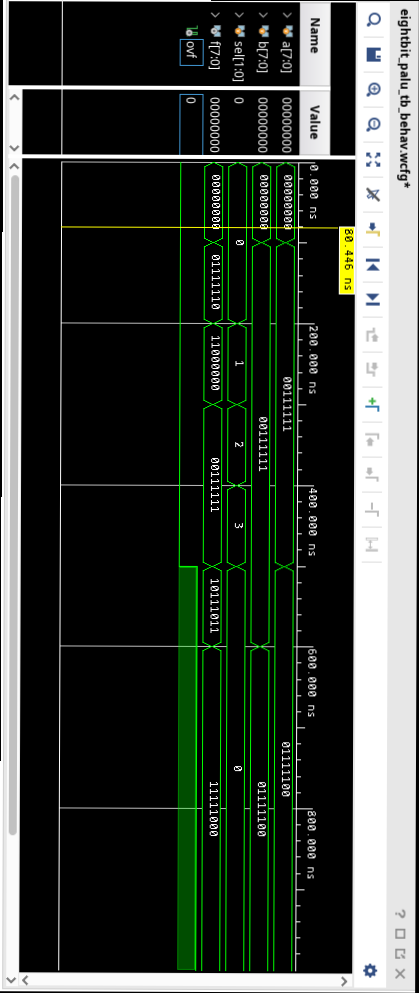
\includegraphics{image}
	\caption{Test bench output}
\end{figure}

\end{document}
